\section{Ergebnis}
Alle nötigen Schritte, um eine Ressource-Grammatik im Grammatical Framework zu implementieren, sind hiermit abgeschlossen. Die Grammatik kann nun geladen und getestet werden. Um die Lateingrammatik zu laden, muss entweder die Datei \textbf{LangLat.gf} oder die Datei \textbf{AllLat.gf} geladen werden. Dies geschieht entweder durch das Aufrufen des Grammatical Frameworks mit der gewünschten Datei als Kommandozeilenparameter (\texttt{\$ gf LangLat.gf} bzw. \texttt{\$ gf AllLat.gf}) oder, wenn die interaktive Eingabeaufforderung des Grammatical Frameworks bereits gestartet ist, durch den Befehl \texttt{> import LangLat.g} bzw. \texttt{> import AllLat.gf}. Die erste dieser Dateien lädt nur die Bestandteile, die alle Sprachen in der Ressource Grammar Library gemein haben, die zweite lädt zusätzlich die sprachspezifische Extra-Grammatik. Ist eine dieser Dateien geladen, kann man die Abhängigkeiten der einzelnen Module betrachten. Wie dieser Abhängigkeitsgraph für die Datei \textbf{AllLat.gf} aussieht, ist in der Grafik \ref{GF-DepGraph} zu sehen. Der Graph für \textbf{LangLat.gf} ist ein Subgraph dieses Graphen, bei dem alle Knoten fehlen, die mit ``All'' und ``Extra'' beginnen. \par
\begin{sidewaysfigure}[h]
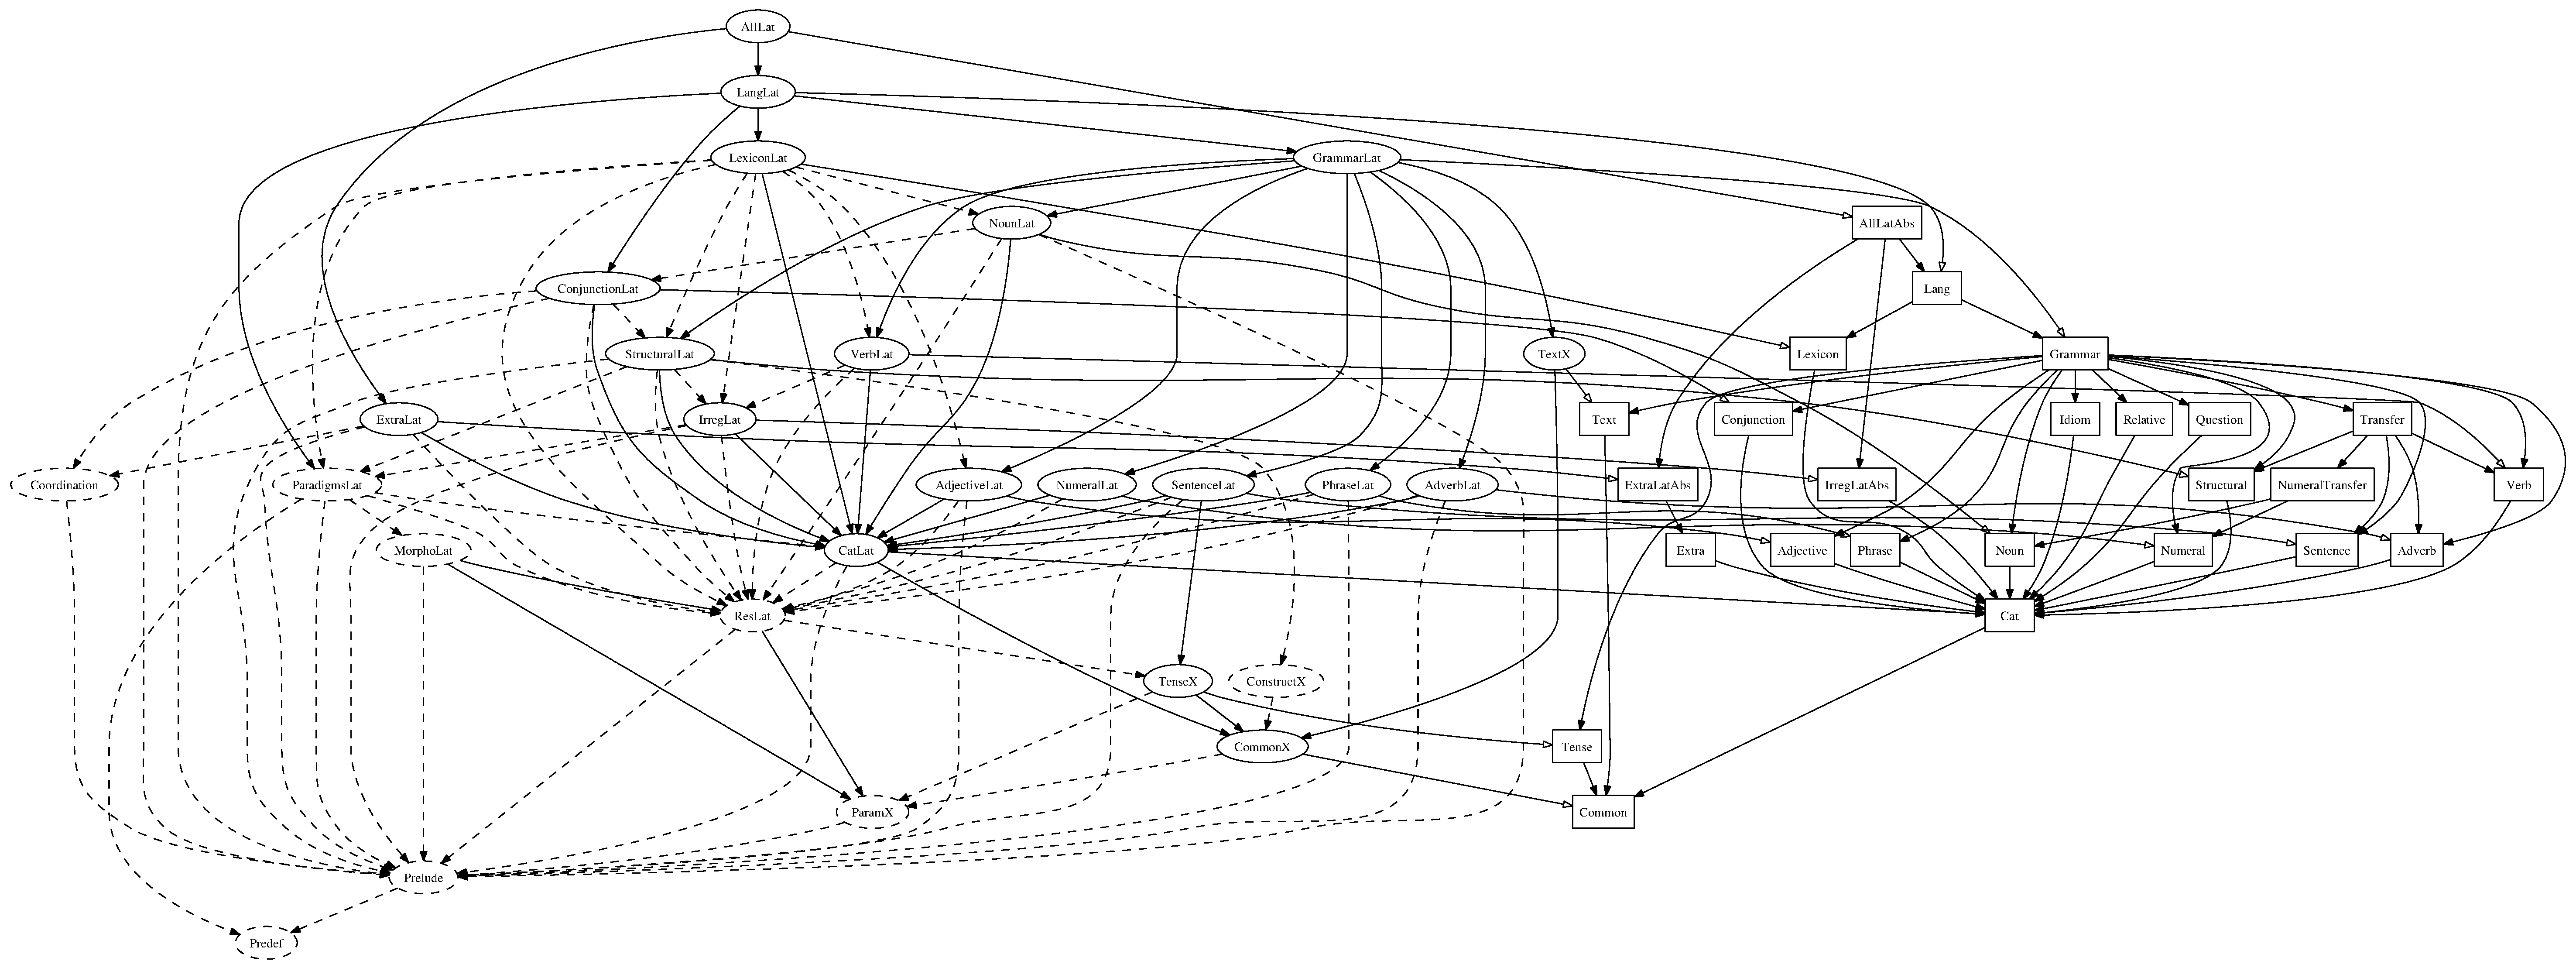
\includegraphics[scale=0.25]{graphics/LatinDependencyGraph.eps}
\caption{Die Abhängigkeiten zwischen den Modulen der Lateingrammatik}\label{GF-DepGraph}
\end{sidewaysfigure}
Nun kann man zum Testen entweder Testsätze parsen oder Sätze anhand der Grammatik erzeugen, um sie auch Korrektheit zu überprüfen. Zum Parsen existiert im Grammatical Framework der offensichtliche Befehl \texttt{parse}, dem eine Zeichenkette als Parameter übergeben wird und als Ergebnis eine Zeichenkette, die die entsprechenden abstrakten Syntaxbäume repräsentiert, zurückgibt. So kann z.B. der Satz \textit{feminae dormiunt} (deutsch: ``Die Frauen schlafen'' bzw. ``Frauen schlafen'') geparsed werden. Als Ergebnis erhält man dann die abstrakten Syntaxbäume in Listing \ref{GF-AbstractStrings}. 
\begin{lstlisting}[float=h!,caption={Abstrakte Syntaxrepräsentationen des Satzes \textit{feminae dormiunt}},label={GF-AbstractStrings},basicstyle=\small]
PhrUtt NoPConj (UttS (UseCl (TTAnt TPres ASimul) PPos (PredVP (DetCN (DetQuant \
  DefArt NumPl) (UseN woman_N)) (UseV sleep_V)))) NoVoc 
PhrUtt NoPConj (UttS (UseCl (TTAnt TPres ASimul) PPos (PredVP (DetCN (DetQuant \
  IndefArt NumPl) (UseN woman_N)) (UseV sleep_V)))) NoVoc
\end{lstlisting}
Mit dem Befehl \texttt{generate\_random} lassen sich dagegen zufällige abstrakte Bäume erzeugen, die mit dem Befehl \texttt{linearize} in einen lateinischen Satz linearisiert werden können. So erzeugt die Befehlsfolge \texttt{> generate\_random | linearize } einen zufälligen lateinischen Satz. Mit dem Befehl \texttt{generate\_trees} können alle Bäume einer Kategorie, bis zu einer gewissen Tiefe, meist der Tiefe von vier, generiert werden. So lassen sich zumindest theoretisch alle in der Grammatik möglichen Sätze bilden. Allerdings sind dies bei dieser Lateingrammatik, selbst bei einer Tiefe von vier, schon fast 70 Millionen Sätze. \par
Offensichtlich ist diese Lateingrammatik also bereits zu einem gewissen Grade benutzbar, jedoch gibt es noch großen Spielraum für Erweiterungen. Die Bereiche des Lexikons und der Morphologie sind bereits komplett entsprechend der abstrakten Syntax, die für eine Ressource Grammar vorgegeben ist, implementiert. Hier wäre es wohl am ehesten sinnvoll, die Ergebnisse, die bereits erzielt werden können zu bewerten, nach möglichen Fehlern zu suchen und diese zu korrigieren. So wären mögliche Fehler im Lexikon z.B. Übersetzungen, die im tatsächlichen Sprachgebrauch fast nie vorkommen oder viel seltener vorkommen als gleichbedeutende Wörter. In diesem Falle sollte die Übersetzung angepasst werden. Fehler in der Morphologie dagegen können dazu führen, dass entweder existierende Wortformen nicht analysiert werden können oder dass Wortformen falsch analysiert werden. Man kann nun unter anderem versuchen, unter Verwendung von Korpora, diese Fehler zu finden. Dies kann jedoch mit lagwieriger Arbeit verbunden sein, die nur unter Umständen nur wenig Verbesserung bringt. \par
Dagegen ist im Bereich der Syntax noch einiges an Arbeit nötig um den vollen Umfang zu erreichen. Viele interessante linguistische Phänomene warten noch darauf, umgesetzt zu werden, denn das Ziel dieser Arbeit war es, überhaupt in der Lage zu sein, lateinische Sätze bilden und analysieren zu können. So fehlen aktuell leider noch Relativsätze, Fragesätze, verschiedene Wortstellungen bei der \texttt{Phr}-Kategorie, Partizipialkonstruktionen, etc. nur um ein paar zu nennen. Dadurch, dass die Anzahl und Funktion der Regeln vorgegeben ist, sollte es aber im Anschluss an diese Arbeit relativ einfach sein, die Grammatik so zu verfollständigen, dass sie als vollständige Sprache in das Grammatical Framework aufgenommen werden kann. 
\section{Anwendung}
Eine Frage der man sich für die Zukunft ebenfalls widmen kann, ist die mögliche Anwendung dieser Lateingrammatik, vor allem, wenn sie in Zukunft noch in den genannten Bereichen erweitert werden sollte. Der Traum jedes Schülers und zugleich wohl der Albtraum der Lehrer wäre ein tatsächlich funktionierendes Lateinübersetzungsprogramm. Ob dieses Ziel, vor allem bei der Übersetzung literarischer und lyrischer Texte, erreicht werden kann, ist jedoch noch nicht abzusehen. Allerdings wäre es denkbar z.B. eine automatisch Übersetzungshilfe für lateinische Inschriften für interessierte Touristen anzubieten. Dafür wäre möglicherweise die Integration in eine Anwendung für moderne Mobiltelefone denkbar. Dies ist insofern möglich, da das Grammatical Framework in der Lage ist Grammatiken in ein portables Grammatikformat umzuwandeln, für das es, teils noch unvollständige, Bibliotheken für verschiedene Programmiersprachen, unter anderem auch Java, gibt. Dadurch ist die Möglichkeit der Benutzung einer PGF-Grammatik in einer Android-Anwendung gegeben. Ebenfalls wäre die Integration in ein Web-Angebot möglich, da auch hierfür Bibliotheken bereitgestellt werden.\footnote{vgl. \cite{RANTA2011} S. 166ff.} \par
Interessanter dürfte jedoch die Überlegung sein, inwieweit diese Lateingrammatik im Unterricht eingesetzt werden könnte. Denn die Verwendung des Computers in der Schule wird wohl auf Dauer zunehmen. Und deshalb müssen für verschiedenste Schulfächer Konzepte zur Einbindung neuer Medien erarbeitet werden, so auch für den Lateinunterricht. Und eben in diesem Bereich sind mögliche Anwendungen dieser Arbeit zu finden. Zum einen ist eine beliebte Beispielanwendung für die Mehrsprachigkeit des Grammatical Frameworks eine Webanwendung namens ``fridge poetry magnets'', bei der man wie aus Magneten am Kühlschrank auf die Wörter gedruckt sind, Sätze bilden kann, die allerdings anders als am Kühlschrank den Regeln einer Grammatik folgen müssen. Die so gebildeten Sätze können dann in verschiedene Sprachen übersetzt werden.\footnote{vgl. \cite{RANTA2011} S. 166} Auf diese Weise ist ein spielerischer Zugang zur lateinischen Sprache möglich, indem man z.B. deutsche Sätze baut und sich anschließend ansehen kann, wie eben dieser Satz auf Latein aussehen würde. Und wegen der Beschränkung, dass nur syntaktisch korrekte Sätze konstruiert werden können, kann man durch das zusammensetzen lateinischer Sätze möglicherweise spielerisch ein Sprachgefühl entwickeln. \par
Außerdem bietet das Grammatical Framework auch Möglichkeiten mit Hilfe einer Grammatik Übungsmöglichkeiten für eine Sprache zu bieten. Denn im Grammatical Framework ist die möglichkeit für sogenannte ``Quizes'' gegeben. Das erste dieser Fragespiele, das mit dem Befehl \texttt{morphology\_quiz} gestartet wird, fragt nach einer spezifischen Wortform eines Wortes einer gegebenen Kategorie, in dem es einem die Grundform und die gewünschten morphologischen Merkmale nennt. Eine Beispielsitzung ist in Listing \ref{GF-MorphoQuiz} zu sehen. Auf diese Weise lässt sich die lateinische Wortformenbildung üben.
\begin{lstlisting}[float=h!,caption={Eine Beispielsitzung des Grammatical Framework Morphology Quiz},label={GF-MorphoQuiz},basicstyle=\small]
> morphology_quiz -cat=N
Welcome to GF Morphology Quiz.
The quiz is over when you have done at least 10 examples
with at least 75 % success.

You can interrupt the quiz by entering a line consisting of a dot ('.').


navis s Pl Voc
> naves
Yes.
Score 1/1
plastica s Pl Nom
> plasticae
Yes.
Score 2/2
pulvis s Sg Voc
>
\end{lstlisting}
Um das Übersetzten auch abseits von Lehrbuchtexten zu üben stellt das Grammatical Framework analog zum ``Morphology Quiz'' ein ``Translation Quiz'' bereit. Um es zu verwenden müssen mindestens die Grammatiken zweier Sprachen geladen sein. Anschließend kann man unter Angabe der Quell- und Zielsprache ähnlich wie bei dem ``Morphology Quiz'' vom Programm vorgegebene Sätze übersetzen, wobei das Können wieder wie oben durch eine Punktzahl bewertet wird. Diese zwei eingebauten Übungsmöglichkeiten sind jedoch nur bedingt für den wirklichen Einsatz im Unterricht geeignet. Da das Grammatical Framework aber leicht in eigene Programme und Systeme integriert werden kann, bieten sich auch hier möglichkeiten zur weiteren Arbeit.\par
In dieser Arbeit wurden die am Anfang beschriebenen Ziele erreicht. Doch wie in diesem Abschnitt dargestellt wurde, bieten sich noch Möglichkeiten um an diese Arbeit anzuknüpfen. Dabei kann man sich entscheiden, ob man sich bemüht die Grammatik weiter zu verbessern oder sich lieber mit der konkreten Umsetzung einer oder mehrerer Verwendungsmöglichkeiten widmet. Für Interessierte bietet diese Arbeit aber auf jeden Fall Anregung und Grundlage für weiterer Beschäftigung.